\documentclass[12pt,a4paper]{article}
\usepackage[left=25mm,right=15mm,top=15mm,bottom=15mm]{geometry}
\usepackage[utf8x]{inputenc}
\usepackage[L7x]{fontenc}
\usepackage[lithuanian]{babel}
\usepackage{url}
\usepackage{float}
\usepackage{graphicx}
\renewcommand{\baselinestretch}{1.2}
\graphicspath{ {img/} }

\begin{document}
\begin{titlepage}
  
  \begin{center}
    \textsc{\LARGE Vilniaus Gedimino Technikos universitetas}\\[2mm]
    \textsc{\Large Elektroninių sistemų katedra}\\[70mm]
    \textsc{\Large Modernios operacinės sistemos}\\[10mm]
    \textsc{\normalsize IBM MIRA}\\[40mm]
    \begin{minipage}{1\textwidth}
      \begin{flushright}
        \emph{Darbą atliko:} Maksim Norkin, AKSfm-15\\
        \emph{Darbą tikrino:} Prof. Vytautas Urbanavičius\\
      \end{flushright}
    \end{minipage}
    \vfill
    {\large Vilnius \\ \the\year}
  \end{center}
\end{titlepage}
\tableofcontents
\newpage

% Juos aprašyti akcentuojant
% Aparatinę įrangą,
% Operacinę sistemą,
% Sprendžiamus uždavinius.

\section{Įvadas}

Objekto padėties nustatymas turi dvi plačias pritaikymo sritis: inercinė navigacinė ir žmogaus judesio sekimo sistema \cite{schlomer2008gesture};

Objekto pozicijos nustatymas, panaudojus inercinius jutiklius remiasi prielaida, jog objektas lieka ramybės būsenoje tol, kol jį nepaveikia išorinė jėga. Tokia jėga suteikia objektui pagreitį. Jeigu rasta pagreitį galima išmatuoti ir suintegruoti, pagreičio ir pozicijos kitimas gali būti išmatuoti. Reikia nepamiršti, kad tokiu atveju matavimą sudarys dvi komponentės -- pagreitis dėl gravitacijos ir išorinės veikiančios jėgos pagreitis. Norint pašalinti gravitacijos komponentę iš pagreičio matavimo, reikia žinoti kokiu kampu akcelerometras yra vertikalės atžvilgiu.
Tokio kampo matavimui, reikalingas kitas jutiklis, kuris vadinasi giroskopas. Jis matuoja kampo greitį, kurį matematiškai integruojant, galima rasti kampo greičio pokytį nuo pradinio, žinomo kampo \cite{sukkarieh2000low}.

Akcelerometras suteikia pagreičio matavimą norimam objektui. Dažniausiai tokie matavimai yra užrašomi $x$, judėjimą tiesiai, $y$, šonu ir $z$ vertikaliai. Giroskopas suteikia matavimus, kurie dengia nurodytas ašis ir yra užrašomi $\theta$, sūkiui, $\beta$ polinkiui ir $\gamma$ vingiavimui, kaip pavaizduota \ref{tikz:axis_of_the_system} pavyzdyje. Tokių inercinių įverčių naudojimas turi pagrindinį privalumą -- stebimo objekto polinkis ir pagreitis gali būti vertinami bet kokioje navigacijoje.  

\begin{figure}[H]
    \centering
    \caption{Objekto pozicijos pagreičio pokyčio ašys, $x$, $y$ ir $z$. Sūkio matmenys apie ašis $\theta$, $\beta$ ir $\gamma$.}
    \label{tikz:axis_of_the_system}
    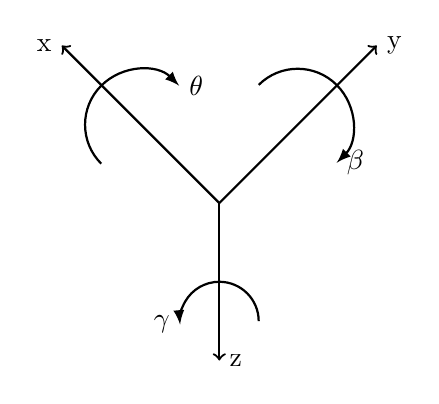
\begin{tikzpicture}
        % axis
        \draw[thick, black, ->] (0,0) -- ( 2, 2) node [right] {y};
        \draw[thick, black, ->] (0,0) -- (-2, 2) node [left] {x}; 
        \draw[thick, black, ->] (0,0) -- ( 0,-2) node [right] {z};
        % arc
        \draw[thick, -latex] ( 0.5,  1.5) arc (135:-45:0.70) node [right] {$\beta$}; 
        \draw[thick, -latex] (-1.5,  0.5) arc (225:45:0.70) node [right] {$\theta$};
        \draw[thick, -latex] ( 0.5, -1.5) arc (0:185:0.5) node [left] {$\gamma$};
    \end{tikzpicture}
\end{figure}

Inercinės navigacijos sistemos yra naudojamos labai plačiai lėktuvuose, raketose, kosmoso laivuose, povandeniniuose ir vandens laivuose \cite{woodman2007introduction}. Progresas gaminant MEMS įrenginius, sudarė galimybes kurti mažas ir lengvas navigacines sistemas. Tokie privalumai leidžia praplatinti įrenginių panaudojimo galimybes ir šiuo metu įtraukia tokias sritis kaip žmogaus ir gyvūnų judesio sekimą.

Tačiau reikia nepamiršti ir apie klaidas, kurias sukelia nuolatinė dedamoji, santykio įverčiai ir nelinijines sistemos įtakos jutiklio verčių nuskaitymo metu. Tokios klaidos yra pagrindinė priežastis atsirasti netikslumams navigacinėje sistemoje per laiko vienetą. Netikslumai sąlygoja akselerometro įverčius, kuriuos tampa labai sunku atskirti tarp gravitacinio lauko ir objekto judėjimo, ko pasekoje objekto pozicijos matavimas toliau yra dar netikslesnis. Kadangi inerciniai jutikliai yra tokio tipo, kuriems yra labai svarbi tiksli prieš tai buvusi pozicija, bet kokia klaida skaičiuojant prieš tai buvusia pozicija, įtakoja ir dabartinės pozicijos skaičiavimą. Tokiu būdu, su laiku navigacinė sistema tampa visiškai netiksli ir praranda visą savo vertę.

\section{Aparatinė įranga}

The Blue Gene/Q sistema yra trečia Blue Gene šeimos kompiuterių architektūros karta \cite{gilge2014ibm}.
Sistema sujungia daugybe komponentų, tarp kurių yra vienas ar daugiau skaičiavimo spintų ir neprivalomi Į/I spintos.
Sistema tankiai susideda iš skaičiavimo mazgų, Į/I spintos ir aptarnavimo kortelės.
Papildoma geležis yra susiejama su saugojimo posisteme, pagrindinis aptarnavimo mazgu (SN), išorinio priėjimo mazgu (FENs) ir komunikacijos posisteme.
Į/I stalčiai, kurie susideda Į/I mazgų, sujungtu su funkciniu vietiniu tinklu (LAN) bendravimui su bylų serveriais, FENs ir SN.
Aptarnavimo kortelės sujungtos su valgymo potinkliu ir yra naudojami SN Blue Gene/Q geležies kontrolei.

Aptarnavimo mazgas pateikia vieną tašką, per kurį galima kontroliuoti ir administruoti Blue Gene/Q sistemą.
Yra įmanoma operuoti sistema, kuri susideda tik iš vieno aptarnavimo mazgo.
Tačiau sistemos aplinka taip pat gali būti sukonfigūruota įtraukti potinklio aptarnavimo mazgus, didesniam plečiamumui.

Priekinio priėjimo mazgui, kuris taip pat vadinamas kaip prisijungimo mazgas, pateikia sistemos resursus, kurie programinės įrangos kūrėjui leidžia prisijungti prie sistemos.
Programuotojai redaguoja ir kompiliuoja programinius paketus, sukuria darbus ir kontrolės bylas, paleidžia darbus sistemoje, nagrinėja gautos programos rezultatus ir atlieka kitus darbus.

Skaičiavimo kortos susideda iš 16 IBM Blue Gene/Q PowerPC A2 branduolio procesorių ir 16 GB darbinės atminties.
Trisdešimt dvi tokios kortos gali būti įtrauktos į mazgo plokštę ir 16 mazgo kortos yra laikomos midplane.
Kompiuterio dėžė gali būti sukonfigūruota dirbti tiek su vienu, tiek su puse midplane.
Sistema gali būti išplėsta iki 512 kompiuterių dėžės.

Kompiuterių dėžių komponentai yra vėsinami arba vandeniu arba oru.
Vanduo yra naudojamas apdorojimo mazguose.
Oras yra naudojamas maitinimo tiekime ir Į/I stalčiuose, kurie yra prijungti prie sistemos.

Į/I stalčiai yra arba atskiros dėžės arba statomos ant kompiuterių dėžių, dažnai vadinamos viršaus kepurės.
Aštuoni Į/I mazgai yra talpinami kiekvienoje iš Į/I stalčių.
Kompiuterinės dėžės yra konfigūruojamos iki keturių Į/I stalčių, du per midplane, naudojant viršutinę kepurę.
Į/I stalčių pozicija Į/I dėžėse yra reguliuojama didelių sistemų diegime, kur Į/I mazgų skaičius negali būti talpinamas spintoje.






\section{Operacinė sistema}

Naudojama operacinė sistema yra ``Compute Node Kernel (CNK)'', kuri yra panaši į Linux ir suteikia naudotojui darbo aplinką leisti procesus \cite{milano2013ibm}.
CNK įtraukia tokias paslaugas:

\begin{itemize}
    \item Proceso sukūrimas ir valdymas
    \item Atminties valdymas
    \item Proceso skrodimas
    \item Patikimumas, pasiekiamumas ir universalumo valdymas
    \item Bylų Į/I
    \item Tinklas
\end{itemize}

Programinis paketas įtraukia į save standartines C/C++ ir Fortran darbo bibliotekas.
Kiek įmanoma, yra palaikomos ir atviro standarto Portable Operacing System Interface (POSIX) sąsajas.
CNK turi grubų gijų palaikymą, kuris įtraukia tokias technologijas kaip pthread, XL OpenMP ir GNU OpenMP.
Native POSIX Thread Library pthreads įgyvendinimas yra palaikomas be modifikacijų.
Statiškai sujungtos paleidžiamos programos pateikia optimalų veikimą, tačiau CNK taip pat palaiko ir dinamiškai sujungtas paleidžiamas programas.
Iš dinamiškai sujungtų programinių programų yra palaikoma tik Python.

\subsection{Į/I mazgų branduolys ir paslaugos}

Į/I mazgas dirba ant branduolio, kuris yra pakeistas Red Hat Enterprise Linux 6 branduolys.
Modifikacija pateikia platformos palaikymą ir didesnį našumą.

Į/I mazgo programinis paketas suteikia Į/I paslaugas skaičiavimo mazgams.
Pavyzdžiui, programos, kurios dirba ant skaičiavimo mazgų gali prieiti prie bylų serverių ir komunikuoti su procesais kitose mašinose.
Į/I mazgai taip pat gali turėti svarbų vaidmenį paleidžiant ir sustabdant darbus ir koordinuojant jų darbą su skrodimo ir stebėjimo įrankiais.

Blue Gene/Q yra be disko sistema, todėl bylų serveriai turi būti.
Aukšto našumo lygiagreti bylų sistema turi būti.
Blue Gene/Q yra labai lanksti ir palaiko skirtingas bylų sistemas, kurias palaiko Linux.
Tipinė lygiagreti bylų sistema yra IBM General Parallel File System (GPFS) ir Lustre.

Į/I magzai įtraukia pilną IP, TCP ir UDP protokolo įgyvendinimus.
Šių protokolų poaibės yra pasiekiamos naudotojo procesams, kurie veikia ant apdorojimo mazgų ir turi susiejimą su Į/I mazgu.
Programos procesai bendrauja su procesais, kurie veikia kituose sistemose per kliento pusės jungtis.
Serverio pusės jungtys taip pat yra palaikomos.
Į/I mazgo jungčių įgyvendinimas yra atliktas tokiu būdu, kad procesai iš apdorojimo mazgų, mano esą tiesiai ant Į/I mazgo.
Tai reiškia, kad jungties port skaičius yra vienas adresas per grupę.
Skaičiavimo mazgai dalinasi Į/I mazgo IP adresu.

Į/I branduolio mazgas yra įgyvendintas taip, kad jis būtų kraunamas kuo rečiau.
Krovimo procesas įtraukia krovimą į darbinę atmintį Linux branduolį ir jo paleidimą iš tos pačios atminties.
Darbinės atminties įkrautas branduolys tuomet yra pateikiamas pradinei bylų sistemai.
Sistema sudedama iš pagrindinių komandų, kurios yra skirtos pakrauti bylų sistemą ant aptarnavimo mazgo per Network File System (NFS).
Krovimas toliau tęsiasi paleisdamas paleidžiant paleidimo programas iš NFS.
Jis taip pat paleidžia naudojo parengtus paleidimo programas, atliekant specifinius veiksmus, kaip pavyzdžiui sistemos pranešimų konfigūracija ir jungimas aukšto našumo bylų sistemas.

Bendros įrankių dėžės bibliotekos ir visi pagrindiniai Linux teksto ir kiauto įrankiai egzistuoja darbinėje atmintyje.
Paketai, kaip pavyzdžiui GPFS, ir naudotojo pateiktos programos yra prijungiamos per NFS ir valdomos su administracinėmis teisėmis.

\subsection{Žinučių perdavimo sąsaja}

Žinučių perdavimo sąsajos įgyvendinimas Blue Gene/Q sistemoje yra MPICH2 standartas, kuris buvo sukurtas Argonne National Labs.

Dinaminis proceso valdymo funkcija yra MPI-2 standartas ir nėra palaikoma Blue Gene/Q sistemos.
Tačiau skirtingi gijų modeliai yra palaikomi.

\subsection{Kompiliatoriai}

Sistemos įrankių dėžės kompiliatoriai ir IBM XL kompiliatoriai Blue Gene/Q skaičiavimo sistemos mazgams yra galimi naudoti iš sistemos.
Kadangi kompiliavimas yra atliekamas priekinio priėjimo mazguose ir ne ant Blue Gene/Q sistemos, yra naudojami daugybės platformos kompiliatoriai.

\subsubsection{GNU kompiliatoriai}

Kompiliatoriai yra paremti GNU šeimos kompiliatoriais.
Kuomet yra diegiamas programinis paketas į sistemą, RPM paketų valdyklė yra suteikiama, kad naudotojai galėtų sukurti su sudiegti įrankių dėžę į \textit{gnu-linux} direktoriją.
Tie patys kompiliatoriai yra panaudoti ir kuriant pačios Blue Gene/Q sistemos programas, todėl yra galimas pilnas bibliotekų palaikymas naudotojo programoms.

\subsubsection{IBM XL kompiliatoriai}

IBM XL kompiliatoriai Blue Gene/Q sistemai gali būti panaudoti programų kompiliavimui.
Kompiliatorius gali sutekti aukštesnio lygio optimizavimo lygį, lyginant su GNU kompiliatoriais.
XL kompiliatoriai palaiko vienos instrukcijos, daugybės duomenų vektorizavimą.
Vektorizavimas suteikia automatinį kodo generavimą ketvirtos eilės slankaus skaičiaus naudojimui.
Toks vienetas vienu metu gali atlaikyti keturias slankaus skaičiaus instrukcijas.
XL kompiliatorius taip pat palaiko išeities kodo sintaksę, kurios pagalba galima skaidriau naudoti atmintį ir spekuliacines gijas.

\subsubsection{MPI apgaubimo programos}

MPI apgaubimo programos yra kompiliatoriaus apgaubimo programos, kurios suteikiamos Blue Gene/Q tvarkyklėje.
Tokios programos gali būti panaudotos kompiliavimui ir sujungimui programų, kurios naudoja MPI.
Skirtinos MPI programos yra galimos, priklausomai nuo panaudoto kompiliatoriaus ir nuo panaudotų bibliotekų versijos.
Apgaubimo programos paleidžia reikalingą kompiliatorių ir sudeda visas reikalingas direktorijas, bibliotekas, ir parametrus, kurie yra reikalingi MPI programos kompiliavimui.
Kiekvienai kompiliavimo kalbai ir Blue Gene/Q standartui, yra atitinkama MPI programa.
Taip pat egzistuoja saugios gijos XL kompiliatoriaus versijos.

\subsection{Programos vystymas ir skrodimas}

Programos vystymo specialistai gali prieiti prie išorinės pusės mazgų, kad sukompiliuoti ir skrosti programas, kurios buvo priskirtos į sistemos darbo režimą ir atlikti kitus interaktyvius veiksmus.

\subsubsection{Skrodimo programos}

Sistema palaiko GNU Project Debugger (GDB) paleidimą su programomis, kurios veikia ant skaičiavimo mazgų.

\subsubsection{Programų paleidimas}

Sistemos programos gali dirbti skirtingais režimais.
Dažniausiai naudojamas metodas yra naudoti darbo planuotoją, kuris palaiko Blue Gene/Q sistemą, kaip pavyzdžiui LoadLeveler planuotojas.
Kita mažiau naudojama alternatyva yra naudoti \textit{runjob} komanda tiesiogiai.
Visi planuotojai naudoja \textit{runjob} sąsaja darbų tvirtinimui, tačiau planuotojai taip pat gali apgaubti darbą su kita komanda arba darbo pridavimo sąsaja.

\subsubsection{Programos atminties sąlygos}

Sistemoje, visa fizinę atmintis ant vieno skaičiavimo mazgo yra $16~GB$, todėl rašant programinį paketą reikia turėti šitą informaciją omenyje.
Kai kuri iš šios atminties jau yra užimta CNK.
Dalinama atminties vieta taip pat yra paskiriama naudotojo procesui, kuomet procesas yra sukuriamas.

CNK seka steko ir kaupo susidūrimus, kuomet kaupas yra plečiamas su \textit{brk()} ir \textit{mmap()} sistemos kvietimais.
CNK ir jos privatūs duomenys yra apsaugomi nuo naudotojo procesų ar gijų skaitymo ir rašymo operacijų.
Proceso kodo erdvė irgi yra apsaugoma nuo kitų procesų ar gijų.
Kodas ir skaitymo duomenys yra padalinami tarp procesų, kurie dalinasi tą patį mazgą.

Atminties dydis, kuris yra reikalingas programai yra svarbus dalykas Blue Gene/Q sistemai.
Naudojama programos atmintis yra klasifikuojama:

\begin{itemize}
    \item bss -- ne inicializuoti statiniai ar paprasti kintamieji
    \item data -- inicializuoti statiniai ar paprasti kintamieji
    \item heap -- kontroliuojamas priskyrimo masyvas
    \item stack -- kontroliuojamas automatinis masyvas ir kintamieji
    \item text -- programos tekstas (instrukcijos) ir skaitymo duomenys
\end{itemize}

Blue Gene/Q sistema palaiko 64 bitų atminties modelį.
Galima naudoti Linux \textit{size} komandą, parodyti programos naudojamą atminties dydį.
Tačiau, \textit{size} komanda neparodo jokios informacijos apie paleisto proceso naudojamos steko ir kaupimo  atminties dydį.

Galimas atminties dydis, kuris yra suteikiamas programai, priklauso nuo procesų skaičiaus viename mazge.
Galimos $16~GB$ atminties dydis yra paskirstomas kaip įmanoma lygiai kiekvienam procesui, kuris dirba ant to mazgo.
Kadangi atmintis yra ribotas resursas, dažniausiai rekomenduojama konservuoti programos atmintį.
Kai kuriais atvejais, atminties reikalavimas gali būti sumažintas paskirstant duomenis, kurie buvo replikuoti originaliam kode.
Tačiau tai reikalauja papildomos komunikacijos.
Sistemoje veikiančių procesų skaičius gali būti labai didelis.
Atmintį galima įsivaizduoti kaip dviejų dimensijų masyvą, kur viena dimensija yra procesų skaičius, o kita dimensija -- galimas atminties laukų skaičius.

\subsubsection{Kiti pastebėjimai}

Labai svarbu yra suprasti, jog operacinė sistema, kuri randasi ant skaičiavimo mazgo nėra pilnas Linux branduolys.
Todėl reikia būti labai atsargiems tokiose operacijose:

\begin{itemize}
    \item Įėjimas ir išėjimas. Labai svarbu kreipti į tai dėmesį. CNK neatlieka jokio Į/I -- viskas yra atliekama Į/I mazgo
    \item Bylų Į/I. Yra palaikoma labai limituota bylų sąsaja. Negalima naudoti asinchroninių bylų operacijų, kadangi tai sukelia klaidų darbo metu
    \item Standartinė įvestis yra palaikoma Blue Gene/Q
    \item Jungčių kvietimai yra palaikoma sistemos
    \item Tiek statinis, tiek dinaminis jungimas yra palaikomas sistemos.
    \item Kiauto programos nėra palaikomos CNK branguolio. Tik paleidžiama programa gali būti startuojama.
    Todėl, jeigu programa reikalauja kiauto programos srautui kontroliuoti, srautas turi būti adaptuojamas.
\end{itemize}


\section{Operacinės sistemos branduolys}

Branduolys suteikia klijus, kuris sujungia visus sistemos komponentus, kad jie galėtų dirbti kartu.
Čia bus apžvelgti pora funkcionalumų, kurie yra įgyvendinti kaip CNK ir Į/I mazgo branduolys, bei informacija apie: skaičiavimo mazgo branduolys, Į/I mazgo branduolio vaidmuo.

\subsection{Skaičiavimo mazgo branduolys}

CNK yra lankstus ir lengvas branduolys Blue Gene/Q sistemos skaičiavimo mazgams, kuris palaiko įvertinimo režimus ir naudojo programas.
Jis suteikia operacinę sistemą, kuri labai panaši į Linux operacinė sistemą ir palaiko platų Linux sistemos palaikomų kvietimų skaičių.
Toks poaibis yra paremtas ant Blue Gene/P sistemos, kuri parodė gerą Linux operacinės sistemos palaikymą ir perkėlimą.
CNK yra optimizuotas specialiai Blue Gene/Q programos specifinei integracinei schemai.

CNK palaiko gijas ir dinaminį sujungimą, kaip dalies Blue Gene/Q sistemos, kuri dar labiau pagerina suderinamumą su Linux operacine sistema.
Kai yra paleidžiama naudojo programa, CNK sujungia Į/I mazgus per torus tinklą.
Toks sujungimas bendrauja per procesus, kurie yra vadinami \textit{Kontroliavimo ir Į/I paslaugos}, kurios dirba ant Į/I mazgo.
Programos lygmenyje, CNK palaiko tokias sąsajas:

\begin{itemize}
    \item Žinučių perdavimo sąsaja tarp skirtingų mazgų, naudojant MPI biblioteką
    \item Atvirą platų apdorojimo sąsaja
    \item Standartizuotus IBM XML šeimos kompiliatorius su XLC/C++, XLF bei GNU šeimos kompiliatorių
    \item Stipriai optimizuotas matematikos bibliotekas, kaip pavyzdžiui IBM inžinerijos ir mokslo paprogrames biblioteka (ESSL)
    \item GNU kompiliatorių rinkinio (GCC) C biblioteka
\end{itemize}

CNK suteikia tokias paslaugas:

\begin{itemize}
    \item Torus tiesioginį atminties priėjimą (DMA), kuris suteikia priėjimą prie skaitymo, rašymo, bei jų dviejų operacijų atminties priėjimą nepriklausomai kiekvienam proceso vienetui. DMA torus sąsaja yra galima naudotojo erdvėje, kas leidžia komunikuoti bibliotekoms ir siųsti žinutes tiesiogiai iš programos, be branduolio įsikišimo. Branduolys su aparatine įranga atlieka saugų registrų limitavimą, kuris draudžia DMA kreiptis į atmintį iš aplikacijos. Tokie limitavimai, kartu su elektroniniu torus skirstymu, suteikia saugumą tarp programų
    \item Bendros atminties priėjimą vietiniam mazge
    \item Aparatinės įrangos konfigūravimą
    \item Atminties valdymą
    \item MPI topologiją
    \item Bylų Į/I
    \item Jungčių sujungimą
    \item Signalus
    \item Gijų valdymą
    \item Torus tinklui transportavimo lygį 
\end{itemize}

\subsubsection{Skaičiavimo mazgo būsena}

Blue Gene/Q aparatinė įranga neturi būsenos -- nėra jokios tik skaitymui skirtos atminties (ROM) ar paprastos Į/I sistemos (BIOS).
Kuomet aparatinė įranga yra perkraunama, sistemos kontrolė turi pakrauti kiekvienam skaičiavimo mazgui operacinę sistemą į atmintį.
Tai yra atliekama per dvi fazes:

\begin{itemize}
    \item Mažas \textit{mikro-programa} komponentas yra pakraunamas į kiekvieno skaičiavimo mazgo darbinę atmintį (RAM). Šis \textit{mikro-programa} paleidžia ir inicializuoja kritines Blue Gene/Q lusto vietas.
    \item Per specializuotą protokolą yra atsiunčiama likusi branduolio dalis. Paskui tos dalys yra paleidžiamos ir šitas paleidimas leidžia prisijungti prie Torus tinklo.
\end{itemize}

\subsubsection{Mikro-programa}

Mikro-programa suteikia žemo lygio galimybių paslaugas tiek Blue Gene specifiniams poreikiams, tiek Linux operacinei sistemai, bei CNK.
Tokia paslauga suteikia patikimą sprendimą per visus mazgus, kartu izoliuojant branduolius nuo kontrolės sistemos įgyvendinimo specifikos.
Paprasčiausio mazgo paslaugos suteikia tą patį žemo lygio aparatinės įrangos paleidimą ir sąsajų paleidimą Linux operacinei sistemai ir skaičiavimo mazgo branduoliui.

\subsection{Į/I branduolio vaidmuo}

Į/I mazgo branduolys suteikia Į/I paslaugas skaičiavimo mazgams ir dirba ant visų Į/I mazgų.
Taip pat mazgas atlieka vaidmenį paleidžiant ir sustabdant darbus, bei koordinavimo veiksmuose su skrodimu ir sekimo įrankiais. Į/I mazgas neturi įtakos programai, tačiau labai verta į jį atkreipti dėmesį, kai yra derinamas Į/I sparta.

\section{Sprendžiami uždaviniai}

Argonne mokslininkai panaudojo Mira super kompiuterį, kad identifikuoti ir patobulinti naują mechanizmą, kuris leidžia pašalinti trintį. To pasekoje pirmą kartą buvo sukurta nauja hibridinė medžiaga, kuri paveldi didelį tepumą makro lygmenyje.

% https://www.sciencedaily.com/releases/2015/07/150721194001.htm
 
Modeliuojami defektai Ni-Al su EAM ir DFT skaičiavimais \cite{0965-0393-24-4-045012}. Atliktas detalus palyginimas tarp įterpto atomo modelio (EAM) ir paskirstymo funkcijos teoremos (DFT) skaičiuojant Ni lydinio defektų sistemas.

Sukimo defektų plačiajuosčiam dažnių diapazone puslaidininkiuose \cite{Seo2016}.

Kaip yra matoma iš pateikiamų straipsnių -- Mira yra naudojamas išskirtinai moksliniams tyrimams, kuriems reikalingos didelės simuliacijos duomenims pasitvirtinti ir prognozuoti.

% http://www.alcf.anl.gov/publications

\section{Išvados}

Šiame darbe buvo aptartai MEMS tipo jutikliai ir galimas jų panaudojimas objekto pozicijos nustatymo procesui. Pradžioje buvo atlikta jutiklių analizė, panagrinėtas pagreičio ir giroskopo jutiklių darbas. Giroskopo atveju, matavimui yra naudojamas vibracinės kilmės elementas, kuris pasiduoda \textit{Coriolis} efektui. Iš šio reiškinio galima nuspręsti kampinio pagreičio pokytį. Pagreičio jutiklio atveju, yra du pagrindiniai įrenginio konstravimo būdai -- mechaniniai ir vibraciniai. Pagrindiniai MEMS tipo jutiklių privalumai prieš kitos formos įtaisus yra mažas dydis, svoris, pigi gamyba (esant dideliems kiekiams), patvari konstrukcija ir mažos galios naudojimas elektriniuose įtaisuose.

Kita medalio pusė yra didelis triukšmų šaltinių skaičius. Nuolatinės komponentės stabilumo, atsitiktinio vaikščiojimo klaidos, poveikis temperatūrai bei kalibravimo klaidos. Tiek pagreičio jutiklis, tiek giroskopas gali veikti gali veikti vibracinio elemento pagrindu. Tokie elementai yra veikiami vibracijos triukšmo ir įvelia į matavimą nukrypimus. Taip pat, bet koks fizinis kūnas reaguoja į temperatūrinius pokyčius. Čia irgi yra triukšmo šaltinis, kadangi prie skirtingų temperatūrų vibracinis elementas vibruoja skirtingai. Tokios problemos kelia iššūkius tyrėjams sugalvoti tokias sistemas, kurios sugeba dirbti kuo efektyviau ir mažinti klaidos įtaka galutiniams skaičiavimams.

Apžvelgti keli darbai, kurių tikslas yra toks pats, tačiau naudojamos visiškai skirtingos metodikos tam tikslui išspręsti. Pirmas nagrinėjimui darbas naudoja tiek pagreičio, tiek kampinio pokyčio jutiklius. Kalibravimas atliekamas matuojant dreifą pirmas $6~s$. Toliau seka duomenų filtravimas, Kalman ir dalelių filtru. Abu filtrai galimai sprendžia navigacinę problemą. Antras darbas remiasi tik pagreičio jutikliu ir naudoja raiškios logikos elementą galutiniam pokyčio įverčiui rasti. Labai svarbu yra pažymėti, jog darbas pasiūlė gerą jutiklių kalibracijos mechanizmą, remiantis gautais rezultatais (\ref{fig:fuzzy_logic_filter} pav.). 

Iš atliktos analizės galima spręsti, jog objekto pozicijos nustatymo sistemos yra reikalingos ir laukiamos rinkoje. Didžiausia kliūtis naudoti tokias sistemas yra įvairūs triukšmai. Tiesiogiai šitų duomenų naudoti modelyje tiesiog nėra galima ir bet kokiu atveju reikia spręsti filtravimo uždavinį.



\newpage

\addcontentsline{toc}{section}{Literatūros ir informacinių šaltinių sąrašas}
\renewcommand\refname{Literatūros ir informacinių šaltinių sąrašas}

\bibliographystyle{plain}
\bibliography{references}

\end{document}